% ============================================================================
%  CHAPITRE 2 -- PROBLÈME, EXIGENCES ET ARCHITECTURE
% ============================================================================
\chapter{Problème, exigences et architecture}
\label{chap:architecture}

\section{Formulation}
\label{sec:formulation}

Soit une image $x \in [0,1]^{3\times H\times W}$ et $n = 3HW$ le nombre de valeurs réelles à transmettre.
L'émetteur dispose de $k$ symboles complexes ; le récepteur produit une reconstruction $\hat{x}$ ou
directement une décision. Deux objectifs s'opposent : la \textbf{fidélité} ($\hat{x}$ ressemble à $x$ au sens
du pixel) et le \textbf{sens} ($\hat{x}$ conduit un système d'analyse indépendant à la même conclusion que
$x$). L'hypothèse du projet est qu'ils ne sont pas équivalents.

\section{Le budget radio}
\label{sec:budget}

Sans budget commun, il suffirait d'accorder plus de bande à un système pour le faire gagner. Le
\textbf{rapport de bande} est donc fixé :
\begin{equation}
  \frac{k}{n} = \frac{\text{symboles complexes émis}}{3HW \text{ valeurs réelles de la source}},
  \qquad \text{point principal : } \frac{k}{n} = \frac{1}{12}.
  \label{eq:kn}
\end{equation}

L'encodeur appris produit 16 canaux latents au stride 4 ; deux valeurs réelles formant un symbole complexe,
transmettre $c$ canaux donne
\begin{equation}
  \frac{k}{n} = \frac{c}{96}, \qquad c \in \{2,4,8,12,16\} \;\Longrightarrow\; \frac{k}{n} \in
  \left\{\tfrac{1}{48}, \tfrac{1}{24}, \tfrac{1}{12}, \tfrac{1}{8}, \tfrac{1}{6}\right\}.
  \label{eq:ratio_c}
\end{equation}

\begin{keybox}[Ce qui varie]
C'est $k$, jamais $n$ : le dénominateur est l'image elle-même. Changer le budget revient à couper des canaux
latents, l'image restant identique. Cette agilité suppose que $c$ soit tiré au hasard à l'entraînement, ce qui
ordonne les canaux par importance : un seul modèle couvre alors les cinq rapports~\cite{kurka2021}.
\end{keybox}

\section{Exigences}
\label{sec:exigences}

\begin{table}[H]
\centering
\caption{Exigences retenues pour que la comparaison soit recevable}
\label{tab:exigences}
\small
\begin{tabularx}{\textwidth}{@{}p{1.1cm}p{4.2cm}>{\raggedright\arraybackslash}X@{}}
\toprule
\textbf{Réf.} & \textbf{Exigence} & \textbf{Mise en œuvre} \\
\midrule
E1 & Budget radio identique & $k$ imposé aux trois chaînes par l'équation~\eqref{eq:kn} \\
E2 & Puissance normalisée à 1 & empêche le gain par amplification ; \srcfile{power_normalize()} \\
E3 & Même canal, mêmes tirages & AWGN et Rayleigh communs, graines fixées par point \\
E4 & Chaîne numérique exacte & chaque paquet codé, modulé, bruité, décodé par Viterbi \\
E5 & Juges indépendants & le classifieur de la perte n'est jamais celui de la mesure \\
E6 & Architecture identique & seule la perte distingue syntaxique et sémantique \\
E7 & Un seul modèle & SNR dans $[0,20]$~dB et bande tirés au hasard à l'entraînement \\
E8 & Reproductibilité & campagne relançable, résultats en CSV, figures régénérées par script \\
\bottomrule
\end{tabularx}
\end{table}

\section{Architecture d'ensemble}
\label{sec:archi}

\begin{figure}[H]
  \centering
  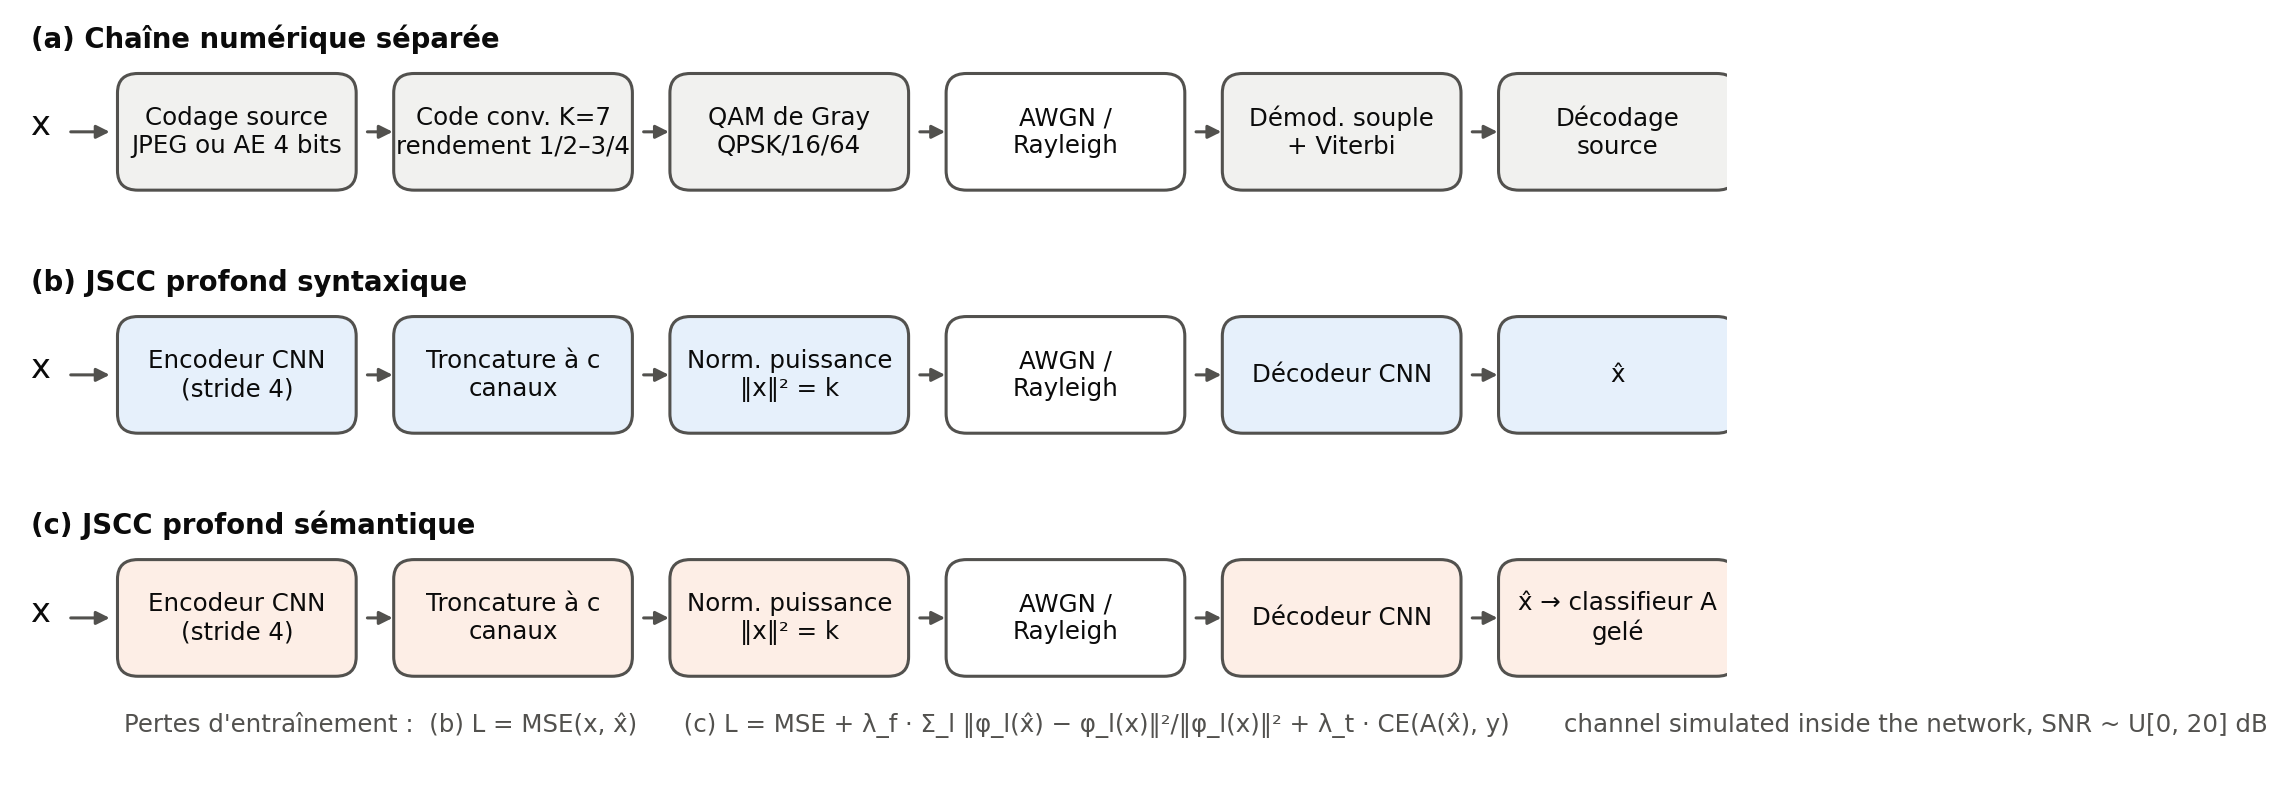
\includegraphics[width=\linewidth]{architecture.png}
  \caption{Les trois systèmes comparés : (a) chaîne numérique séparée, (b) JSCC syntaxique entraîné sur une
  perte pixel, (c) JSCC sémantique, de même architecture, entraîné avec les termes de caractéristiques et de
  tâche. Le canal simulé est commun aux trois.}
  \label{fig:architecture}
\end{figure}

\section{Organisation logicielle}
\label{sec:logiciel}

\begin{table}[H]
\centering
\caption{Organisation du code (Python et PyTorch)}
\label{tab:code}
\small
\begin{tabularx}{\textwidth}{@{}p{3.6cm}>{\raggedright\arraybackslash}X@{}}
\toprule
\textbf{Module} & \textbf{Contenu} \\
\midrule
\srcfile{semcom/channel.py} & normalisation de puissance, AWGN, Rayleigh avec égalisation ZF, troncature \\
\srcfile{semcom/models.py} & encodeur et décodeur JSCC, auto-encodeur 4 bits, classifieurs A et B, modèle de tâche \\
\srcfile{semcom/digital.py} & code convolutif, poinçonnage, QAM de Gray, LLR, Viterbi, débit JPEG \\
\srcfile{semcom/metrics.py} & PSNR, SSIM, métriques sémantiques ResNet-18 \\
\srcfile{semcom/data.py} & chargeurs CIFAR-10, Kodak et Y4M \\
\srcfile{semcom/train.py} & boucles d'entraînement, description des neuf modèles \\
\srcfile{semcom/video.py} & transmission image par image et renouvellement conditionnel \\
\srcfile{scripts/} & données, entraînement, évaluation, figures, démonstration, simulateur \\
\srcfile{explorer/} & simulateur interactif (chapitre~\ref{chap:simulateur}) \\
\bottomrule
\end{tabularx}
\end{table}

Tous les modèles d'image sont \textbf{entièrement convolutifs} : un réseau entraîné en $32\times32$
s'applique sans modification à des images $768\times512$ ou à des trames $352\times288$, pourvu que les
dimensions soient divisibles par 4. C'est ce qui rend possible l'évaluation par transfert du
chapitre~\ref{chap:resultats}.
